\section{Experiments}
\label{sec:experiments}

\subsection{Setup}
\label{sec:exp-setup}

\textbf{Models.} Five dense decoder-only LLMs spanning the Llama-3, Falcon3 and Mistral lineages and
the $3$B--$24$B range:
\textbf{Llama-3.2-3B}~\citep{dubey2024llama3}, \textbf{Falcon3-7B}~\citep{falcon3},
\textbf{Llama-3.1-8B-Instruct}~\citep{dubey2024llama3},
\textbf{Mistral-Nemo-12B}~\citep{mistralnemo2407} and
\textbf{Mistral-Small-24B}~\citep{mistralsmall2501}. Four are base pretrained checkpoints and one is
instruction-tuned, so the comparison spans both regimes; all use grouped-query attention, so
attention units are KV-aligned query-head groups.

\textbf{Benchmarks.} We follow the evaluation protocol established for training-free structured
pruning~\citep{ma2023llmpruner,an2024flap,ling2024slimgpt,tang2025slimllm}: language-modelling
perplexity together with zero-shot multiple-choice accuracy. Perplexity is measured on
WikiText-2~\citep{merity2017wikitext}, PTB~\citep{marcus1993ptb} and C4~\citep{raffel2020c4} at a
$2048$-token context. Accuracy is measured on twelve benchmarks covering commonsense reasoning
(PIQA~\citep{bisk2020piqa}, HellaSwag~\citep{zellers2019hellaswag},
WinoGrande~\citep{sakaguchi2021winogrande}, CommonsenseQA~\citep{talmor2019commonsenseqa}), science
question answering (ARC-easy/challenge~\citep{clark2018arc},
OpenBookQA~\citep{mihaylov2018openbookqa}), reading comprehension (BoolQ~\citep{clark2019boolq},
RACE and RACE-high~\citep{lai2017race}, QuAIL~\citep{rogers2020quail}) and world knowledge
(MMLU~\citep{hendrycks2021mmlu}). Every task is scored on its \emph{full} test set through one
shared harness (\cref{app:protocol}).

We report both families, and it is worth saying at the outset which one carries which claim. Perplexity
is how this literature compares methods, and we report it so our numbers are readable against published
ones; it is also the family our objective is closest to. But a language-modelling loss can miss
capability damage --- \cref{sec:exp-analysis} exhibits a mask that improves WikiText while losing double
digits on every capability group --- so we never let a perplexity win stand in for a capability claim.
Where the two families disagree we say so and let the accuracy columns decide. The result is that the
lead does not rest on the weaker witness: it is present in both families at once.

\textbf{Baselines.} Seven training-free baselines under identical budgets and harness:
\textbf{Random}, \textbf{Magnitude}~\citep{han2015learning}, \textbf{Wanda-sp}~\citep{sun2024wanda,an2024flap},
\textbf{FLAP}~\citep{an2024flap}, \textbf{LLM-Pruner}~\citep{ma2023llmpruner},
\textbf{SlimGPT}~\citep{ling2024slimgpt} and \textbf{SlimLLM}~\citep{tang2025slimllm}.
\Cref{app:baselines} adds two more on the headline model: \textbf{AMP}~\citep{sultan2025amp} inside the
same guard, and the two-stage \textbf{2SSP}~\citep{sandri2025twossp} under its own per-layer budget,
because its two stages are the method. The regime is \emph{selection-only}: the question is which units to remove, so post-pruning weight
repair and fine-tuning are disabled for every method including ours, namely LLM-Pruner's
LoRA~\citep{hu2022lora}, SlimLLM's regression update, SlimGPT's OBS update and FLAP's bias
compensation. \Cref{sec:exp-recovery} adds an identical LoRA stage to
every selection at once.

\textbf{Protocol.} Calibration is $128$ sequences of C4 (the Wanda/SparseGPT convention), from which
we build $\Hmat$ with top-$r{=}256$ logits and $16$ FFN groups per layer; every calibration-based
baseline receives that same set. Cost is non-embedding parameters, and the same cost vector
defines the budget for every method. Every method is pruned under one guard, a per-layer cap of $1.5\rho$ with the first and last two
layers protected, and every mask must realise its target ratio to within $0.2$ points to be reported:
a run outside that band is not at the operating point its column names and is excluded from the
comparison. $\hat\lambda$ is re-derived at each model and ratio from $16$ held-out
sequences by \cref{eq:lambdahat}, with no benchmark consulted. Every configuration is fixed in
advance and shared by all methods (\cref{app:protocol}).

% ============================== Table 1: two-ratio headline ==============================
% Generated by scripts/make_tables.py -- do not edit by hand.
% Float and caption only; numbers are generated into tab_headline_shaded.tex.
\begin{table}[t]
\centering
\caption{\textbf{Llama-3.1-8B-Instruct, all reported tasks.} Eight training-free methods under one
guard and one harness, each realising its target ratio to within $0.2$ points, on full test sets.
Shading is rank within a column among the pruned methods, darkest best.}
\label{tab:headline}
\resizebox{\textwidth}{!}{% generated by scripts/make_shaded_tables.py -- do not edit by hand
\begin{tabular}{llccccccccccccccc}
\toprule
 & & \multicolumn{3}{c}{LM perplexity $\downarrow$} & \multicolumn{4}{c}{Commonsense $\uparrow$} & \multicolumn{3}{c}{Science QA $\uparrow$} & \multicolumn{4}{c}{Reading $\uparrow$} & \multicolumn{1}{c}{Know. $\uparrow$} \\
\cmidrule(lr){3-5}\cmidrule(lr){6-9}\cmidrule(lr){10-12}\cmidrule(lr){13-16}\cmidrule(lr){17-17}
 $\rho$ & Method & Wiki & PTB & C4 & PIQA & HellaS & WinoG & CSQA & ARC-e & ARC-c & OBQA & BoolQ & RACE & RACE-h & QuAIL & MMLU \\
\midrule
 -- & Dense & 6.40 & 10.36 & 10.67 & 80.9 & 77.4 & 66.2 & 59.2 & 78.1 & 54.4 & 47.6 & 85.0 & 68.8 & 54.1 & 62.7 & 47.8 \\
\midrule
 \multirow{8}{*}{20\%} & SlimLLM & \cellc{71}{17.36} & \cellc{57}{30.59} & \cellc{43}{29.36} & \cellc{86}{75.2} & \cellc{71}{60.0} & \cellc{43}{56.2} & \cellc{57}{47.6} & \cellc{100}{65.2} & \cellc{86}{39.5} & \cellc{100}{39.8} & \cellc{43}{65.8} & \cellc{57}{51.3} & \cellc{71}{39.4} & \cellc{57}{47.8} & \cellc{86}{37.2} \\
  & SlimGPT & \cellc{57}{19.24} & \cellc{14}{35.52} & \cellc{57}{29.19} & \cellc{43}{73.4} & \cellc{43}{58.8} & \cellc{57}{56.6} & \cellc{29}{44.6} & \cellc{43}{61.9} & \cellc{43}{37.4} & \cellc{29}{35.4} & \cellc{0}{64.3} & \cellc{14}{47.8} & \cellc{14}{36.6} & \cellc{0}{44.5} & \cellc{29}{35.1} \\
  & LLM-Pruner & \cellc{86}{13.23} & \cellc{100}{19.36} & \cellc{86}{21.98} & \cellc{71}{75.0} & \cellc{86}{64.6} & \cellc{86}{57.4} & \cellc{100}{51.8} & \cellc{29}{60.4} & \cellc{29}{37.2} & \cellc{57}{36.8} & \cellc{100}{79.1} & \cellc{86}{57.2} & \cellc{100}{45.2} & \cellc{86}{52.4} & \cellc{71}{36.8} \\
  & FLAP & \cellc{14}{20.88} & \cellc{0}{36.77} & \cellc{71}{29.06} & \cellc{29}{73.2} & \cellc{57}{59.0} & \cellc{14}{54.9} & \cellc{43}{46.7} & \cellc{86}{62.5} & \cellc{57}{37.7} & \cellc{71}{38.2} & \cellc{57}{70.9} & \cellc{29}{49.9} & \cellc{57}{39.2} & \cellc{14}{45.6} & \cellc{43}{35.3} \\
  & Wanda-sp & \cellc{43}{20.02} & \cellc{29}{35.29} & \cellc{29}{30.09} & \cellc{57}{73.7} & \cellc{29}{57.4} & \cellc{71}{57.0} & \cellc{71}{48.9} & \cellc{57}{62.5} & \cellc{71}{38.8} & \cellc{43}{36.4} & \cellc{71}{72.2} & \cellc{71}{52.8} & \cellc{29}{38.7} & \cellc{29}{46.6} & \cellc{57}{35.6} \\
  & Magnitude & \cellc{29}{20.49} & \cellc{43}{31.38} & \cellc{14}{34.93} & \cellc{14}{68.9} & \cellc{14}{55.5} & \cellc{29}{55.9} & \cellc{14}{41.7} & \cellc{14}{54.6} & \cellc{14}{31.4} & \cellc{14}{32.4} & \cellc{14}{65.2} & \cellc{43}{50.2} & \cellc{43}{39.1} & \cellc{71}{49.4} & \cellc{14}{32.8} \\
  & Random & \cellc{0}{21.20} & \cellc{71}{30.44} & \cellc{0}{36.77} & \cellc{0}{68.2} & \cellc{0}{53.8} & \cellc{0}{54.5} & \cellc{0}{38.5} & \cellc{0}{50.3} & \cellc{0}{29.4} & \cellc{0}{31.4} & \cellc{29}{65.4} & \cellc{0}{47.1} & \cellc{0}{36.1} & \cellc{57}{47.8} & \cellc{0}{31.8} \\
  & \textbf{CoCurve} & \cellc{100}{12.88} & \cellc{86}{29.63} & \cellc{100}{19.58} & \cellc{100}{75.8} & \cellc{100}{67.5} & \cellc{100}{61.0} & \cellc{86}{50.4} & \cellc{86}{62.5} & \cellc{100}{41.9} & \cellc{86}{39.6} & \cellc{86}{78.3} & \cellc{100}{58.1} & \cellc{86}{44.0} & \cellc{100}{54.1} & \cellc{100}{38.5} \\
\midrule
 \multirow{8}{*}{30\%} & SlimLLM & \cellc{43}{78.23} & \cellc{43}{100.68} & \cellc{29}{109.42} & \cellc{71}{69.5} & \cellc{14}{37.8} & \cellc{29}{52.0} & \cellc{71}{36.9} & \cellc{86}{53.0} & \cellc{71}{28.8} & \cellc{71}{28.2} & \cellc{71}{62.5} & \cellc{29}{35.9} & \cellc{29}{29.4} & \cellc{29}{37.2} & \cellc{71}{30.4} \\
  & SlimGPT & \cellc{14}{196.79} & \cellc{14}{317.47} & \cellc{14}{208.42} & \cellc{29}{62.1} & \cellc{43}{38.9} & \cellc{14}{51.2} & \cellc{29}{30.4} & \cellc{29}{42.8} & \cellc{43}{25.4} & \cellc{43}{27.4} & \cellc{57}{51.3} & \cellc{14}{35.4} & \cellc{29}{29.4} & \cellc{43}{38.0} & \cellc{14}{27.9} \\
  & LLM-Pruner & \cellc{86}{26.64} & \cellc{86}{39.70} & \cellc{86}{40.31} & \cellc{100}{71.0} & \cellc{86}{54.4} & \cellc{43}{52.4} & \cellc{100}{43.2} & \cellc{71}{51.0} & \cellc{86}{33.2} & \cellc{86}{30.4} & \cellc{100}{73.4} & \cellc{100}{48.4} & \cellc{100}{38.8} & \cellc{86}{47.8} & \cellc{86}{31.9} \\
  & FLAP & \cellc{29}{79.37} & \cellc{29}{177.67} & \cellc{43}{102.06} & \cellc{57}{65.7} & \cellc{71}{41.0} & \cellc{86}{53.6} & \cellc{43}{33.5} & \cellc{43}{43.8} & \cellc{14}{24.8} & \cellc{29}{26.8} & \cellc{29}{51.2} & \cellc{43}{37.8} & \cellc{71}{32.0} & \cellc{29}{37.2} & \cellc{43}{29.0} \\
  & Wanda-sp & \cellc{57}{61.15} & \cellc{57}{94.85} & \cellc{71}{87.17} & \cellc{57}{65.7} & \cellc{29}{38.5} & \cellc{57}{53.4} & \cellc{57}{33.7} & \cellc{57}{45.8} & \cellc{57}{27.8} & \cellc{71}{28.2} & \cellc{0}{47.7} & \cellc{71}{41.9} & \cellc{43}{31.0} & \cellc{57}{40.1} & \cellc{57}{29.6} \\
  & Magnitude & \cellc{0}{324.46} & \cellc{0}{642.26} & \cellc{0}{273.86} & \cellc{0}{57.0} & \cellc{0}{32.2} & \cellc{0}{51.0} & \cellc{0}{24.7} & \cellc{0}{31.5} & \cellc{29}{25.0} & \cellc{0}{25.6} & \cellc{57}{51.3} & \cellc{0}{33.1} & \cellc{0}{28.8} & \cellc{0}{34.8} & \cellc{0}{27.3} \\
  & Random & \cellc{71}{52.90} & \cellc{71}{84.29} & \cellc{57}{87.88} & \cellc{14}{60.6} & \cellc{57}{40.2} & \cellc{71}{53.5} & \cellc{14}{29.6} & \cellc{14}{41.0} & \cellc{0}{24.1} & \cellc{14}{26.6} & \cellc{14}{47.8} & \cellc{57}{41.4} & \cellc{57}{31.8} & \cellc{71}{42.6} & \cellc{29}{28.6} \\
  & \textbf{CoCurve} & \cellc{100}{21.59} & \cellc{100}{36.31} & \cellc{100}{31.99} & \cellc{86}{70.5} & \cellc{100}{55.8} & \cellc{100}{55.5} & \cellc{86}{41.0} & \cellc{100}{55.6} & \cellc{100}{34.4} & \cellc{100}{35.2} & \cellc{86}{73.1} & \cellc{86}{46.5} & \cellc{86}{37.3} & \cellc{100}{50.1} & \cellc{100}{33.4} \\
\midrule
 \multirow{8}{*}{40\%} & SlimLLM & \cellc{71}{183.53} & \cellc{71}{211.36} & \cellc{71}{217.27} & \cellc{71}{62.6} & \cellc{71}{31.2} & \cellc{43}{50.4} & \cellc{71}{29.2} & \cellc{100}{41.6} & \cellc{57}{24.0} & \cellc{43}{25.0} & \cellc{71}{51.2} & \cellc{57}{31.6} & \cellc{71}{27.3} & \cellc{57}{32.1} & \cellc{71}{27.6} \\
  & SlimGPT & \cellc{29}{26002} & \cellc{0}{32398} & \cellc{29}{13079} & \cellc{14}{51.9} & \cellc{29}{26.2} & \cellc{29}{49.2} & \cellc{14}{21.0} & \cellc{14}{27.9} & \cellc{43}{23.9} & \cellc{86}{29.2} & \cellc{0}{38.2} & \cellc{0}{25.3} & \cellc{57}{26.7} & \cellc{0}{21.1} & \cellc{57}{26.9} \\
  & LLM-Pruner & \cellc{86}{103.35} & \cellc{86}{165.07} & \cellc{86}{125.68} & \cellc{100}{65.3} & \cellc{100}{42.7} & \cellc{100}{52.2} & \cellc{100}{33.4} & \cellc{71}{40.0} & \cellc{86}{28.1} & \cellc{57}{26.8} & \cellc{100}{65.1} & \cellc{86}{36.0} & \cellc{86}{32.2} & \cellc{86}{40.2} & \cellc{100}{29.7} \\
  & FLAP & \cellc{0}{49940} & \cellc{14}{29989} & \cellc{14}{13823} & \cellc{29}{52.1} & \cellc{14}{26.0} & \cellc{29}{49.2} & \cellc{29}{22.0} & \cellc{29}{28.0} & \cellc{29}{23.5} & \cellc{0}{22.6} & \cellc{29}{41.6} & \cellc{29}{26.6} & \cellc{0}{25.4} & \cellc{14}{23.3} & \cellc{0}{25.6} \\
  & Wanda-sp & \cellc{57}{1015} & \cellc{57}{1288} & \cellc{57}{860.91} & \cellc{57}{54.8} & \cellc{43}{26.3} & \cellc{0}{48.2} & \cellc{57}{25.6} & \cellc{57}{33.1} & \cellc{0}{22.4} & \cellc{14}{22.8} & \cellc{14}{38.7} & \cellc{43}{27.8} & \cellc{29}{26.0} & \cellc{43}{24.8} & \cellc{29}{26.6} \\
  & Magnitude & \cellc{14}{27101} & \cellc{29}{23937} & \cellc{0}{13834} & \cellc{0}{51.1} & \cellc{0}{25.4} & \cellc{71}{50.8} & \cellc{0}{19.0} & \cellc{0}{25.7} & \cellc{71}{25.9} & \cellc{71}{27.8} & \cellc{57}{48.2} & \cellc{14}{25.6} & \cellc{14}{25.8} & \cellc{29}{24.4} & \cellc{14}{26.2} \\
  & Random & \cellc{43}{4168} & \cellc{43}{3201} & \cellc{43}{3152} & \cellc{43}{54.0} & \cellc{57}{29.0} & \cellc{57}{50.5} & \cellc{43}{24.1} & \cellc{43}{31.3} & \cellc{14}{23.4} & \cellc{29}{24.0} & \cellc{43}{42.5} & \cellc{71}{33.3} & \cellc{43}{26.4} & \cellc{71}{35.4} & \cellc{43}{26.7} \\
  & \textbf{CoCurve} & \cellc{100}{59.13} & \cellc{100}{108.37} & \cellc{100}{76.05} & \cellc{86}{64.0} & \cellc{86}{41.0} & \cellc{86}{51.4} & \cellc{86}{31.9} & \cellc{86}{41.6} & \cellc{100}{28.7} & \cellc{100}{29.6} & \cellc{86}{62.3} & \cellc{100}{41.9} & \cellc{100}{32.2} & \cellc{100}{42.8} & \cellc{86}{29.3} \\
\bottomrule
\end{tabular}
}
\end{table}


\subsection{Main results}
\label{sec:exp-main}

\textbf{The gap opens as compression bites.} \Cref{tab:headline} reports the headline model task by
task. Across the three budgets it is
first or second in \emph{all forty-five} columns, and first in twenty-seven of them; the best competitor
reaches thirteen of fifteen in its strongest block and no other method exceeds five. At $30\%$ \method
holds ten of the fifteen columns outright --- all three perplexities and seven of the twelve accuracy
tasks, including world knowledge and both science benchmarks. Our WikiText margin over the best baseline widens monotonically with the budget on this model, from
$2.6\%$ at $20\%$ to $19.0\%$ at $30\%$ and $42.8\%$ at $40\%$. A coupling account predicts exactly this. While a model is
over-parameterised, almost any $20\%$ of its units can go without the survivors having to compensate.
Once the budget forces removals that genuinely depend on one another, the term that models that
dependence decides whether the remaining network still computes anything. Nothing about the method
changes across the sweep: the same objective, estimator and solver, with $\hat\lambda$ re-derived at
each ratio by \cref{eq:lambdahat} rather than scheduled. On Falcon3-7B it returns $0.218$ at $20\%$
and $0.149$ at $30\%$ without ever being shown the ratio.

\textbf{The advantage holds across five models and three scales.} \Cref{tab:cross-model} compares
each model against a strict bar: the per-column best of every baseline run for it --- a bar that in ten
of the fifteen blocks no single competitor attains, and that in the other five LLM-Pruner attains
alone. The envelope carries all seven baselines on thirteen of the fifteen model--ratio blocks,
Mistral-Small-24B included at every ratio; the two that carry fewer are itemised with their reasons in
\cref{app:baselines}.
Against that envelope \method leads on $38$ of the $45$ perplexity cells and
$32$ of the $60$ capability-group cells. The envelope is a hard bar on the second of those:
it is attained by LLM-Pruner in $70\%$ of them, so beating it there is essentially beating the one
baseline in the set that backpropagates through the whole model. It is also one of the two that do not
run at $24$B in published form: LLM-Pruner needs $94.3$\,GB of device memory against an $80$\,GB card,
and SlimGPT $344$\,GB of host memory against $128$\,GB, and both are in the table there only because we
re-implemented them to stream (\cref{tab:selcost}). Against the seven taken one at a time, \method leads
in $666$ of $721$ cells. Five of the seven take under one cell in twenty; the two that do better are
SlimLLM at $13\%$ and LLM-Pruner at $27\%$.

Perplexity margins are easier to read along the ratio axis than the quality axis. Interpolating each
model's baseline envelope over the five measured ratios, the perplexity \method delivers at
$\rho{=}30$--$40\%$ is the perplexity the strongest baseline reaches $2.2$ to $6.6$ points of
compression earlier. That holds on nine of the ten model--ratio points; the exception is
Llama-3.2-3B at $\rho{=}40\%$. \Cref{fig:pareto} extends this to the full sweep.

Mistral-Small-24B makes the point most sharply, and it makes it along the ratio axis. At
$\rho{=}20\%$ a $24$B model has slack to spare, and the field is correspondingly tight: we take C4 and
the envelope takes WikiText and PTB, all three within a few tenths of a point on a model whose dense
WikiText is $4.70$. That is the same observation as the widening margin above, seen from the end where
there is not yet anything to choose. At $\rho{=}30\%$ its perplexity is $20.5$ against the strongest
baseline's $78.8$ --- a $3.8\times$ margin --- while four of the seven are above $470$: at that ratio it
is the only method on that model still holding a usable perplexity. At $\rho{=}40\%$ the margin is $11.9\times$, $277.1$ against the
best of all seven baselines, Random at $3299$; the next two are SlimLLM at $3969$ and LLM-Pruner at
$5495$, and SlimGPT lands at $9057$. The direction reverses on the
smallest model: at $\rho{=}40\%$ Llama-3.2-3B loses every cell to the envelope --- its three perplexity
columns to SlimLLM and three of its four capability groups to LLM-Pruner, though against LLM-Pruner
alone we still lead on PTB and C4. That is the ratio at which a $3$B model stops having an allocation
worth choosing: the best of the eight methods there is already $19.7\times$ dense perplexity, so the
block records which of two unusable models is nominally ahead.

\textbf{The objective delivers what it optimises.} The criterion is token-level KL to the dense model,
so the pruned model should reproduce the dense model's decisions more faithfully than the alternatives
do. It does. At $\rho{=}30\%$ on Llama-3.1-8B-Instruct, \method matches the dense prediction more often
than any baseline on three of six tasks, and is a close second on the rest, with every baseline but one
behind it everywhere. \Cref{app:fidelity} breaks this down and relates it to where the two metrics of
\cref{tab:cross-model} diverge.

\textbf{The per-task columns show what an average hides.} A pruned model collects a floor of $0.375$ on the seven-task mean for answering nothing, so it can post
a respectable average while having stopped answering several of its tasks. That is what has happened to
the field at $30\%$: three of seven baselines are at or below chance on ARC-challenge, and five of
seven are at or below the majority-class rate on BoolQ. \method is above chance on all twelve tasks at
every ratio in \cref{tab:headline}.

\textbf{The result does not depend on the field we compare against, the prompt format, or the
precision.} Three checks, reported in full in the appendix, ask whether the lead is an artefact of the
setup that produced it. Widening the field to nine competitors, including the two most recent selectors,
AMP and 2SSP, leaves the ordering intact: \method is first on seven of the eleven task columns and on
the commonsense average, and second on two more (\cref{tab:main-8b}). Replacing the zero-shot prompt
with five demonstrations --- the regime in which damage to attention shows first, and the reason SlimGPT
and 2SSP both report it --- leaves it first on both models at both ratios (\cref{tab:fewshot}).
Quantising the pruned model to $4$ bits costs it about what the same step costs the dense model in
accuracy, so the two compressions draw on different slack rather than the same slack twice
(\cref{app:quant}). And the criterion's own target is met: among the nine methods, ours reproduces the
dense model's predictions most faithfully, first or second on all six tasks measured
(\cref{app:fidelity}).

% ============================== Table 2: cross-model summary ==============================
% Generated by scripts/make_tables.py -- do not edit by hand.
% Float and caption only; numbers are generated into tab_cross.tex.
\begin{table}[t]
\centering
\caption{\textbf{Five models, three shared ratios.} ``Best base.'' is the per-column best of the
training-free baselines run for that model: each baseline's own group average is taken first, then
the best baseline for that column. \textbf{Bold} is the better of the two rows, in whichever row it
falls; the blue band marks our row, and its intensity is the size of our margin where we lead. Groups
average PIQA/HellaSwag/WinoGrande/CSQA, ARC-e/ARC-c/OBQA, and BoolQ/RACE/RACE-h/QuAIL. Per-method
numbers: \cref{tab:full-unified}.}
\label{tab:cross-model}
{\small% generated by scripts/make_cross_table.py -- do not edit by hand
\setlength{\tabcolsep}{4pt}\renewcommand{\arraystretch}{0.98}
\begin{tabular}{@{}lllrrrrrrr@{}}
\toprule
 & & & \multicolumn{3}{c}{Perplexity $\downarrow$} & \multicolumn{4}{c}{Accuracy $\uparrow$} \\
\cmidrule(lr){4-6}\cmidrule(l){7-10}
 Model & $\rho$ & & Wiki & PTB & C4 & Cmn. & Sci. & Read. & Know. \\
\midrule
 Llama-3.2-3B & 20\% & Best base. & 16.90 & 29.84 & 24.64 & 55.4 & 40.8 & 45.3 & 33.5 \\
\rowours & & \textbf{CoCurve} & \cellc{5}{\textbf{16.66}} & \cellc{28}{\textbf{27.34}} & \cellc{19}{\textbf{23.24}} & \cellc{7}{\textbf{56.6}} & \cellc{13}{\textbf{42.4}} & \cellc{32}{\textbf{49.7}} & \cellc{4}{\textbf{33.9}} \\
\addlinespace[1.5pt]
  & 30\% & Best base. & 42.69 & 54.64 & \textbf{50.48} & \textbf{48.5} & 33.7 & 43.5 & 29.5 \\
\rowours & & \textbf{CoCurve} & \cellc{62}{\textbf{34.78}} & \cellc{32}{\textbf{49.40}} & 55.02 & 48.2 & \cellc{16}{\textbf{35.3}} & \cellc{5}{\textbf{44.2}} & \cellc{6}{\textbf{30.0}} \\
\addlinespace[1.5pt]
  & 40\% & Best base. & \textbf{136.1} & \textbf{159.8} & \textbf{130.0} & \textbf{43.7} & \textbf{30.3} & \textbf{39.7} & \textbf{28.0} \\
\rowours & & \textbf{CoCurve} & 193.7 & 256.5 & 196.5 & 40.2 & 28.5 & 37.9 & 26.8 \\
\midrule
 Falcon3-7B & 20\% & Best base. & 7.43 & 12.62 & 16.49 & \textbf{60.0} & \textbf{48.3} & \textbf{55.0} & \textbf{39.8} \\
\rowours & & \textbf{CoCurve} & \cellc{16}{\textbf{7.07}} & \cellc{24}{\textbf{11.72}} & \cellc{17}{\textbf{15.65}} & 59.4 & 48.1 & 53.8 & 37.8 \\
\addlinespace[1.5pt]
  & 30\% & Best base. & 10.07 & 17.65 & 22.34 & 55.3 & 41.0 & \textbf{50.6} & 34.8 \\
\rowours & & \textbf{CoCurve} & \cellc{38}{\textbf{8.92}} & \cellc{49}{\textbf{15.05}} & \cellc{43}{\textbf{19.47}} & \cellc{6}{\textbf{56.3}} & \cellc{13}{\textbf{42.6}} & 49.2 & \cellc{9}{\textbf{35.8}} \\
\addlinespace[1.5pt]
  & 40\% & Best base. & 18.36 & 28.74 & 37.94 & \textbf{49.7} & 35.2 & \textbf{46.5} & 31.1 \\
\rowours & & \textbf{CoCurve} & \cellc{82}{\textbf{13.83}} & \cellc{65}{\textbf{23.11}} & \cellc{77}{\textbf{29.21}} & 49.5 & \cellc{9}{\textbf{36.1}} & 45.3 & \cellc{5}{\textbf{31.6}} \\
\midrule
 Llama-3.1-8B-It & 20\% & Best base. & 13.23 & \textbf{19.36} & 21.98 & 62.2 & \textbf{48.2} & 58.5 & 37.2 \\
\rowours & & \textbf{CoCurve} & \cellc{9}{\textbf{12.88}} & 29.63 & \cellc{36}{\textbf{19.58}} & \cellc{8}{\textbf{63.7}} & 48.0 & \cellc{1}{\textbf{58.6}} & \cellc{11}{\textbf{38.5}} \\
\addlinespace[1.5pt]
  & 30\% & Best base. & 26.64 & 39.70 & 40.31 & 55.2 & 38.2 & \textbf{52.1} & 31.9 \\
\rowours & & \textbf{CoCurve} & \cellc{63}{\textbf{21.59}} & \cellc{28}{\textbf{36.31}} & \cellc{69}{\textbf{31.99}} & \cellc{3}{\textbf{55.7}} & \cellc{31}{\textbf{41.7}} & 51.8 & \cellc{16}{\textbf{33.4}} \\
\addlinespace[1.5pt]
  & 40\% & Best base. & 103.3 & 165.1 & 125.7 & \textbf{48.4} & 31.6 & 43.4 & \textbf{29.7} \\
\rowours & & \textbf{CoCurve} & \cellc{100}{\textbf{59.13}} & \cellc{100}{\textbf{108.4}} & \cellc{100}{\textbf{76.05}} & 47.1 & \cellc{17}{\textbf{33.3}} & \cellc{11}{\textbf{44.8}} & 29.3 \\
\midrule
 Mistral-Nemo-12B & 20\% & Best base. & 11.44 & 175.7 & 17.83 & 60.1 & 46.7 & 51.4 & 35.6 \\
\rowours & & \textbf{CoCurve} & \cellc{82}{\textbf{8.63}} & \cellc{100}{\textbf{83.37}} & \cellc{66}{\textbf{14.31}} & \cellc{11}{\textbf{62.1}} & \cellc{22}{\textbf{49.7}} & \cellc{34}{\textbf{56.7}} & \cellc{12}{\textbf{36.9}} \\
\addlinespace[1.5pt]
  & 30\% & Best base. & 17.75 & 164.5 & 24.84 & \textbf{57.2} & \textbf{42.9} & \textbf{50.5} & \textbf{33.0} \\
\rowours & & \textbf{CoCurve} & \cellc{38}{\textbf{15.75}} & \cellc{8}{\textbf{160.4}} & \cellc{21}{\textbf{23.27}} & 56.1 & 40.8 & 49.4 & 31.7 \\
\addlinespace[1.5pt]
  & 40\% & Best base. & 73.06 & 499.3 & 86.26 & \textbf{48.8} & \textbf{35.0} & \textbf{45.9} & \textbf{30.0} \\
\rowours & & \textbf{CoCurve} & \cellc{95}{\textbf{52.20}} & \cellc{29}{\textbf{455.4}} & \cellc{59}{\textbf{71.01}} & 48.2 & 32.4 & 44.5 & 29.3 \\
\midrule
 Mistral-Small-24B & 20\% & Best base. & \textbf{8.71} & \textbf{69.46} & 15.35 & 67.0 & 55.2 & 59.8 & \textbf{43.7} \\
\rowours & & \textbf{CoCurve} & 8.97 & 131.2 & \cellc{10}{\textbf{14.88}} & \cellc{4}{\textbf{67.8}} & \cellc{7}{\textbf{56.3}} & \cellc{6}{\textbf{60.9}} & 43.5 \\
\addlinespace[1.5pt]
  & 30\% & Best base. & 78.78 & 464.7 & 116.4 & 58.5 & \textbf{49.8} & 51.5 & 36.5 \\
\rowours & & \textbf{CoCurve} & \cellc{100}{\textbf{20.49}} & \cellc{33}{\textbf{419.1}} & \cellc{100}{\textbf{29.67}} & \cellc{4}{\textbf{59.3}} & 48.2 & \cellc{17}{\textbf{54.1}} & \cellc{0}{\textbf{36.5}} \\
\addlinespace[1.5pt]
  & 40\% & Best base. & 3299 & 4747 & 1271 & \textbf{45.1} & \textbf{37.6} & 34.1 & 30.0 \\
\rowours & & \textbf{CoCurve} & \cellc{100}{\textbf{277.1}} & \cellc{50}{\textbf{4037}} & \cellc{100}{\textbf{231.6}} & 44.3 & 33.1 & \cellc{75}{\textbf{41.8}} & \cellc{0}{\textbf{30.0}} \\
\bottomrule
\end{tabular}
}
\end{table}


\begin{figure}[t]
\centering
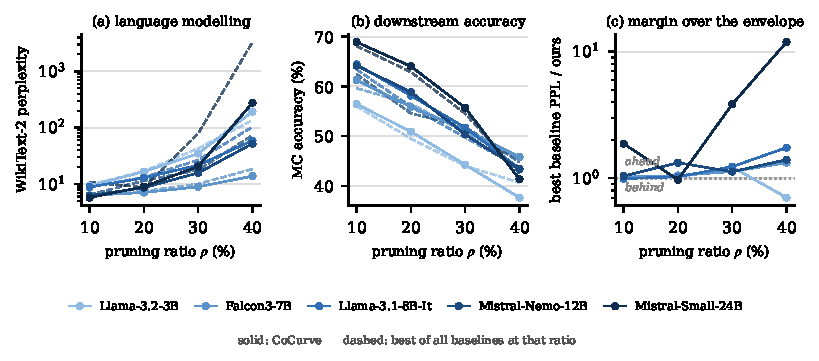
\includegraphics[width=\textwidth]{figures/fig_ratio_sweep.pdf}
\caption{\textbf{Across ratios and scales.} Solid: \method. Dashed: the best of all baselines at that
ratio, an envelope rather than one competitor. (c) is (a) as a ratio; above one is ahead. The margin
widens with compression on Falcon3-7B, Llama-3.1-8B-Instruct and Mistral-Small-24B, reaching $11.9\times$ at $40\%$ on the last. The panels stop at $\rho{=}40\%$ because at $50\%$ the
axis stops separating methods rather than favouring one: in \cref{tab:ratio-full} every method measured
at $\rho{=}50\%$ is at least $7.6\times$ dense perplexity, and on four of the five models even the best
of them is past $100\times$.}
\label{fig:pareto}
\end{figure}

\subsection{Ablations: what the edge term buys}
\label{sec:exp-ablation}

The gain is the off-diagonal, not the diagonal it sits on and not the module split it happens to
move. \Cref{tab:ablation} tests all three readings at once on ten models spanning six families: one
measurement, paired over the same sixteen held-out sequences, in three pairs of columns.

\begin{table}[t]
\centering\footnotesize
\caption{\textbf{The off-diagonal is what pays, and how much to trust it has to be measured}
($\rho{=}20\%$, $16$ held-out sequences at the $2048$-token deployment length). $|\mathcal{F}|$ is
the number of distinct prunings in the enumerated family; $\hat\lambda$ is the selected segment.
$\Delta$ is how much \emph{worse} each alternative is than $\hat\lambda$, with $\sigma$ its paired
standard errors. Right-hand block: the attention/FFN split is frozen at the diagonal selector's own
allocation, so the two arms remove identical cost of each type and only the ordering can differ.
Rows are ordered by size; on the two Qwen models the selected segment begins at exactly
$\lambda{=}0$, so the criterion keeps the diagonal solution and $\sigma$ is undefined.}
\label{tab:ablation}
% generated by scripts/make_ablation_table.py -- do not edit by hand
\footnotesize\setlength{\tabcolsep}{3pt}\renewcommand{\arraystretch}{1.02}
\begin{tabular}{@{}l c c cc cc cc@{}}
\toprule
& & & \multicolumn{2}{c}{$\lambda{=}0$} & \multicolumn{2}{c}{$\lambda{=}1$} & \multicolumn{2}{c}{split frozen}\\
\cmidrule(lr){4-5}\cmidrule(lr){6-7}\cmidrule(l){8-9}
Model & $|\mathcal{F}|$ & $\hat\lambda$ & $\Delta$\% & $\sigma$ & $\Delta$\% & $\sigma$ & $\Delta$\% & $\sigma$\\
\midrule
Llama-3.2-3B & 288 & $0.0911$ & +9.6 & 3.3 & +12.4 & 3.8 & +11.5 & 4.2\\
Falcon3-7B & 181 & $0.218$ & +6.6 & 8.2 & +29.7 & 23.1 & +7.6 & 11.4\\
Mistral-7B & 318 & $0.0165$ & +5.8 & 5.9 & +32.0 & 11.0 & -- & --\\
Qwen2.5-7B & 115 & $\mathbf{0}$ & +0.0 & -- & +6.7 & 4.7 & -- & --\\
Llama-3.1-8B-It & 303 & $0.0108$ & +6.7 & 4.6 & +13.0 & 6.0 & +8.5 & 5.4\\
Yi-1.5-9B & 400 & $0.0141$ & +3.8 & 2.1 & +746.9 & 39.1 & +4.4 & 3.1\\
Falcon3-10B & 402 & $0.0126$ & +2.5 & 3.9 & +30.1 & 8.3 & -- & --\\
Mistral-Nemo-12B & 371 & $2.4{\cdot}10^{-4}$ & +0.4 & 3.1 & +32.2 & 17.1 & +0.9 & 2.7\\
Llama-2-13B & 553 & $1.2{\cdot}10^{-5}$ & +0.1 & 1.4 & +94.7 & 21.5 & -- & --\\
Qwen2.5-14B & 716 & $\mathbf{0}$ & +0.0 & -- & +22.2 & 13.9 & -- & --\\
\bottomrule
\end{tabular}

\end{table}

\textbf{Removing the edges costs, and never gains.} Setting $\lambda\!=\!0$ deletes the off-diagonal and reduces \method to an OBD-style diagonal saliency
(\cref{eq:decomp}) that shares everything else: the same $\Hmat$ diagonal, cost normalisation, budget
and guard. The path rejects it on eight of ten models, by up to $9.6\%$ of held-out risk and $8.2$
paired standard errors, and the differences are paired over the same held-out sequences, so sequence
difficulty cancels rather than being averaged away. The gap carries downstream: on
Llama-3.1-8B-Instruct at the same cap and realised ratio the diagonal selector reaches MMLU $.373$
against $.385$, a gap of $1.2$ points, against the at most $0.81$ that redrawing the
calibration set moves any capability group (\cref{app:seed-variance}). On the remaining two models the selected segment begins at $\lambda\!=\!0$, and
the procedure returns the diagonal selector unchanged rather than something worse.

\textbf{Trusting them fully costs more.} Taking the whole off-diagonal at face value,
$\lambda\!=\!1$, is rejected on \emph{every} model, by $6.7\%$ to $747\%$ and at $3.8$ to $39.1$
paired standard errors. How far to trust the off-diagonal is therefore a measurement, and a
method that asserts $\lambda{=}1$ without measuring is wrong on ten models out of ten, and one that
asserts $\lambda{=}0$ is wrong on eight of them.

\textbf{And the gain is a reordering, not a re-split.} $\lambda$ also moves how the shared budget divides between attention and FFN. We therefore freeze that
division at the \emph{diagonal} selector's own per-type budget, a quantity any OBD-style method
produces without our matrix, and re-derive $\hat\lambda$ inside the constraint. Both arms then remove
identical attention and FFN cost by construction, and the $\lambda\!=\!0$ member of the constrained
family \emph{is} the diagonal selector. An interior $\hat\lambda$ still wins on every model we ran it
on, by $2.7$ to $11.4$ paired standard errors. The same conclusion survives coarser and finer
interaction granularity (\cref{tab:granularity}), a resampled held-out set and three alternative
selection rules (\cref{app:lambda-robust}), and rebuilding $\Hmat$ from disjoint calibration text
(\cref{app:seed-variance}). Restricting the eligible units to a single module type
costs wherever the restriction binds: on Llama-3.2-3B both restrictions cost, and an attention-only
budget cannot reach $20\%$ at all on Falcon3-7B, which has four attention units per layer. On that
model the objective spends nothing on attention of its own accord, so the FFN-only arm \emph{is} the
joint arm (\cref{tab:singlemodule}).

\subsection{Efficiency}
\label{sec:exp-efficiency}

Compression is worth its accuracy cost only if it buys speed, so we measure it on physically removed
units rather than masks (\cref{tab:efficiency}): every timing runs on sliced weight matrices rather
than masked full-size ones (\cref{app:units}). Removing $40\%$ of the non-embedding parameters gives
a $1.40\times$ prefill speedup at $0.66\times$ peak memory on Llama-3.2-3B and $1.49\times$ at
$0.66\times$ on Llama-3.1-8B-Instruct, and leaves $0.62\times$ the parameters at $0.63\times$ peak
memory on Mistral-Small-24B. At a
fixed removed fraction, structured methods land in one narrow band --- \cref{tab:efficiency-band} times all
eight methods at $\rho{=}20\%$ on one machine and their prefill speedups span $1.13$ to $1.19\times$.
What a method is worth is therefore the accuracy it delivers at that speedup (\cref{tab:headline},
\cref{tab:cross-model}). Selection cost
does differ between methods, and \cref{app:selection-cost} reports it.

% Body efficiency table: what compression buys, on physically removed units. The cross-method
% comparison is one sentence in the text (every structured method lands in the same band) rather
% than eight near-identical rows, which is how SlimLLM and 2SSP report the same thing. Every number
% here is measured; ratios not measured are not shown.
\begin{table}[t]
\centering\small
\caption{\textbf{What compression buys}, measured on physically removed units rather than masks
(one RTX 6000 Ada, bf16, eager attention, on an otherwise idle machine; the $24$B row is
timed the same way on one A100-80GB, which is the card that holds it dense). Throughput is relative to
dense, and \emph{Params} is the ratio of total parameters, so a $20\%$ non-embedding removal reads
below $1$ but not at $0.80$. At a fixed removed fraction every structured method lands in the same
band: prefill $1.17$--$1.21\times$ at $\rho{=}20\%$ across the four architectures timed here, and on
the headline model the eight methods sit within $0.07$\,GB of each other on peak memory. The axis on
which methods differ is therefore accuracy at a given speedup, not the speedup.}
\label{tab:efficiency}
\adjustbox{max width=\textwidth}{% generated by scripts/make_efficiency_table.py -- do not edit by hand
\footnotesize
\setlength{\tabcolsep}{7pt}\renewcommand{\arraystretch}{1.02}
\begin{tabular}{@{}l r rrrr@{}}
\toprule
Model & Removed & Params\dn & Prefill\up & Decode\up & Peak mem\dn \\
\midrule
Llama-3.2-3B & $20\%$ & $0.82\times$ & $1.17\times$ & $1.10\times$ & $0.83\times$ \\
Falcon3-7B & $20\%$ & $0.82\times$ & $1.19\times$ & $1.16\times$ & $0.83\times$ \\
Llama-3.1-8B-Instruct & $20\%$ & $0.83\times$ & $1.17\times$ & $1.06\times$ & $0.83\times$ \\
Mistral-Nemo-12B & $20\%$ & $0.82\times$ & $1.21\times$ & $1.18\times$ & $0.82\times$ \\
\midrule
Llama-3.2-3B & $40\%$ & $0.65\times$ & $1.40\times$ & $1.09\times$ & $0.66\times$ \\
Llama-3.1-8B-Instruct & $40\%$ & $0.65\times$ & $1.49\times$ & $1.22\times$ & $0.66\times$ \\
\rowours Mistral-Small-24B & $40\%$ & $0.62\times$ & \textemdash & \textemdash & $0.63\times$ \\
\bottomrule
\end{tabular}
}
\end{table}



\subsection{With a light recovery stage}
\label{sec:exp-recovery}

Past roughly $40\%$, no training-free method leaves a model within reach of dense accuracy. A
practitioner then asks what a short recovery stage buys, and whether a better selection still matters
once weights are allowed to move. One experiment answers both. We apply an identical LoRA stage, at the
same rank, token budget, schedule and corpus, to \method and to four baselines at each of three ratios.
The corpus is disjoint from the calibration set. These models are no longer training-free, so we report
them separately from every other number in this paper (\cref{tab:recovery}).

Recovery compresses the field, as it should --- a random selection, once tuned, finishes above at least
two tuned baselines at every ratio, which is a caution against reading tuned numbers as evidence about
selection. What survives the compression is the ordering: \method holds the best value in $15$ of the
$18$ cells, and after tuning it has the highest seven-set commonsense average at all three ratios, by
$0.2$, $1.8$ and $1.5$ points. A short recovery stage therefore does not substitute for choosing well; it starts from
wherever the selection left the model.

% Generated by scripts/make_tables.py -- do not edit by hand.
% Float and caption only; numbers are generated into tab_recovery_shaded.tex.
\begin{table}[t]
\centering
\caption{\textbf{Selection quality survives recovery} (Llama-3.1-8B-Instruct). The same five
selections before and after one identical LoRA stage --- same rank, token budget, schedule and corpus,
on a corpus disjoint from the calibration set. $\text{Cmn}_7$ is the seven-set commonsense
average conventional in the pruning literature (ARC-e/c, HellaSwag, WinoGrande, PIQA, OBQA, BoolQ) ---
a wider set than the four-task Cmn group of \cref{tab:headline} --- and Ret.\% is the fraction of the
dense model's $\text{Cmn}_7$ retained. Shading is rank within a column.}
\label{tab:recovery}
{\footnotesize% generated by scripts/make_recovery_table.py -- do not edit by hand
\setlength{\tabcolsep}{4pt}\renewcommand{\arraystretch}{0.95}
\begin{tabular}{@{}llrrrrrr@{}}
\toprule
 & & \multicolumn{3}{c}{w/o tune (training-free)} & \multicolumn{3}{c}{w/ tune (LoRA)} \\
\cmidrule(lr){3-5}\cmidrule(l){6-8}
 $\rho$ & Method & Wiki$\downarrow$ & $\mathrm{Cmn}_7\uparrow$ & Ret.\% & Wiki$\downarrow$ & $\mathrm{Cmn}_7\uparrow$ & Ret.\% \\
\midrule
 -- & Dense & 6.40 & 70.2 & 100.0 & \multicolumn{3}{c}{--} \\
\midrule
 \multirow{5}{*}{20\%} & SlimLLM & \cellc{50}{17.36} & \cellc{50}{57.5} & \cellc{50}{81.9} & \cellc{50}{10.17} & \cellc{50}{62.0} & \cellc{50}{88.3} \\
  & SlimGPT & \cellc{25}{19.24} & \cellc{25}{55.5} & \cellc{25}{79.0} & \cellc{25}{10.88} & \cellc{25}{61.9} & \cellc{25}{88.1} \\
  & LLM-Pruner & \cellc{75}{13.23} & \cellc{75}{58.7} & \cellc{75}{83.7} & \cellc{100}{9.86} & \cellc{0}{61.3} & \cellc{0}{87.4} \\
  & Random & \cellc{0}{21.20} & \cellc{0}{50.5} & \cellc{0}{72.0} & \cellc{0}{11.32} & \cellc{75}{62.4} & \cellc{75}{89.0} \\
  & \textbf{CoCurve} & \cellc{100}{12.88} & \cellc{100}{61.0} & \cellc{100}{87.0} & \cellc{75}{10.04} & \cellc{100}{62.6} & \cellc{100}{89.2} \\
\midrule
 \multirow{5}{*}{30\%} & SlimLLM & \cellc{25}{78.23} & \cellc{50}{47.4} & \cellc{50}{67.6} & \cellc{50}{13.93} & \cellc{25}{56.3} & \cellc{25}{80.2} \\
  & SlimGPT & \cellc{0}{196.79} & \cellc{25}{42.8} & \cellc{25}{61.0} & \cellc{25}{14.69} & \cellc{75}{57.1} & \cellc{75}{81.4} \\
  & LLM-Pruner & \cellc{75}{26.64} & \cellc{75}{52.2} & \cellc{75}{74.4} & \cellc{75}{13.01} & \cellc{0}{55.2} & \cellc{0}{78.6} \\
  & Random & \cellc{50}{52.90} & \cellc{0}{42.1} & \cellc{0}{60.0} & \cellc{0}{15.29} & \cellc{50}{56.8} & \cellc{50}{80.9} \\
  & \textbf{CoCurve} & \cellc{100}{21.59} & \cellc{100}{54.3} & \cellc{100}{77.4} & \cellc{100}{12.64} & \cellc{100}{58.9} & \cellc{100}{83.9} \\
\midrule
 \multirow{5}{*}{40\%} & SlimLLM & \cellc{50}{183.53} & \cellc{50}{40.8} & \cellc{50}{58.2} & \cellc{50}{19.61} & \cellc{25}{51.9} & \cellc{25}{74.0} \\
  & SlimGPT & \cellc{0}{26002} & \cellc{0}{35.2} & \cellc{0}{50.2} & \cellc{0}{24.27} & \cellc{0}{50.4} & \cellc{0}{71.8} \\
  & LLM-Pruner & \cellc{75}{103.35} & \cellc{100}{45.7} & \cellc{100}{65.1} & \cellc{75}{17.43} & \cellc{50}{52.1} & \cellc{50}{74.2} \\
  & Random & \cellc{25}{4168} & \cellc{25}{36.4} & \cellc{25}{51.8} & \cellc{25}{20.04} & \cellc{75}{52.2} & \cellc{75}{74.4} \\
  & \textbf{CoCurve} & \cellc{100}{59.13} & \cellc{75}{45.5} & \cellc{75}{64.8} & \cellc{100}{16.33} & \cellc{100}{53.7} & \cellc{100}{76.5} \\
\bottomrule
\end{tabular}
}
\end{table}


\subsection{Beyond one tower: vision--language models}
\label{sec:exp-vlm}

Nothing in \cref{sec:method} is specific to a decoder-only stack. The risk is a KL divergence between
a frozen model and a masked copy of it; the estimator is a Gram matrix of single-unit ablation
features; the selector is a cost-normalised greedy under one budget. Point those three objects at a
vision--language model and the only thing that changes is that the unit inventory grows a second
tower. Everything else is held fixed: the same $M$ single-unit ablations, the same
$\Hmat_{uv}=\bar{D}_u^{\top}\bar{D}_v/P$, the same $\lambda$ protocol of \cref{sec:method-lambda}, the
same guard, no gradients, no fine-tuning and no adapter. One piece of bookkeeping is new --- the layer
index is composite, so the per-layer cap treats a vision layer and a language layer as distinct
layers rather than pooling them --- and it introduces no hyperparameter.

\textbf{Protocol.} The table below reports \vlmNcolsW\ vision--language models spanning $2$B to
$8$B and three model families --- Qwen2-VL \citep{wang2024qwen2vl}, Qwen2.5-VL
\citep{bai2025qwen25vl}, Qwen3-VL \citep{qwen3vl2025}, InternVL3 \citep{zhu2025internvl3} and
LLaVA-1.5 \citep{liu2024llava15}; the full grid of \vlmGridModelsW\ models at three ratios, adding
LLaVA-NeXT \citep{liu2024llavanext}, is in \cref{app:vlm}, on the
seven benchmarks this literature reports as a matter of course --- MMBench-EN
\citep{liu2024mmbench}, SEED-Bench \citep{li2024seedbench}, ScienceQA-IMG \citep{lu2022scienceqa},
AI2D \citep{kembhavi2016ai2d}, MMStar \citep{chen2024mmstar}, POPE \citep{li2023pope} and MME
\citep{fu2023mme} --- at $1000$ items each, with the dense model measured
under our own harness rather than quoted. Calibration is a fixed draw of Flickr30k image--caption pairs
\citep{young2014flickr30k}, whose images are disjoint from the COCO-derived suites by construction;
\cref{app:vlm} gives the draw for each model. The baselines are the
training-free structured selectors this field returns to: Magnitude \citep{han2015learning},
Wanda-sp \citep{sun2024wanda}, FLAP \citep{an2024flap}, LLM-Pruner's gradient Taylor score
\citep{ma2023llmpruner}, a ShortGPT-style layer drop \citep{men2024shortgpt}, and Random. Every arm receives the identical
budget, guard, calibration draw and scoring code; the only thing that differs between rows is which
units get removed. \Cref{app:vlm} gives the per-benchmark breakdown and every configuration measured.

\begin{table}[t]
\centering\small
\caption{Vision--language models, mean accuracy over seven benchmarks at $1000$ items each. Every
selector is training-free and runs under one shared budget and one shared guard. Retention is
floor-corrected against the dense model measured here.}
\label{tab:vlm}
% Five model groups plus the widest row label ("diagonal only") run 44pt past the text block at the
% default column separation. Tightening the gutter fits it without shrinking the type.
\setlength{\tabcolsep}{2pt}
\begin{tabular}{@{}lccccc@{}}
\toprule
 & \multicolumn{1}{c}{Qwen2-VL-2B} & \multicolumn{1}{c}{Qwen2.5-VL-7B} & \multicolumn{1}{c}{Qwen3-VL-8B} & \multicolumn{1}{c}{InternVL3-8B} & \multicolumn{1}{c}{LLaVA-1.5-7B} \\
\cmidrule(lr){2-2}\cmidrule(lr){3-3}\cmidrule(lr){4-4}\cmidrule(lr){5-5}\cmidrule(lr){6-6}
Selector & $20\%$ & $20\%$ & $20\%$ & $20\%$ & $20\%$ \\
\midrule
Dense (no pruning) & 73.0 & 81.6 & 83.4 & 83.6 & 64.1 \\
\midrule
\textbf{\method} & \textbf{59.3} & \textbf{74.4} & \textbf{71.1} & \textbf{75.9} & \textbf{57.1} \\
\quad diagonal only ($\lambda{=}0$) & 53.7 & 73.5 & 66.5 & 73.9 & 50.0 \\
\midrule
LLM-Pruner & 57.0 & 72.2 & 65.8 & 71.8 & 53.7 \\
Wanda-sp & 51.5 & 62.9 & 40.5 & 49.8 & 36.0 \\
FLAP & 36.6 & 73.3 & 68.4 & 74.8 & 41.1 \\
ShortGPT (layer drop) & 35.5 & 35.3 & 35.2 & 43.4 & 34.6 \\
Magnitude & 40.3 & 72.9 & 57.0 & 70.7 & 48.1 \\
Random & 48.0 & 64.4 & 53.8 & 67.9 & 52.8 \\
\midrule
\emph{\method retention of dense} & 66\% & 86\% & 76\% & 85\% & 78\% \\
\bottomrule
\end{tabular}

\end{table}

\textbf{Result.} \method leads every baseline in all \vlmNcolsW\ columns, by \vlmMarginLo\ to
\vlmMarginHi\ points of seven-benchmark mean, and is first outright in \vlmNfirst\ of the
\vlmNcells\ per-benchmark cells against a standard error of $\vlmSE$ points. No single baseline is the
one being beaten: the runner-up is \vlmRunnerUps. Because the budget is shared and the objective is
cost-normalised, the split between towers is an output rather than a hyperparameter: on the five
models whose vision tower holds under a tenth of the removable parameters it spends nothing there at
all, and on Qwen2-VL-2B, where the vision tower holds a third of them, it takes a fifth of the budget
from the vision side. Nothing in the objective was told to do either.

\textbf{Along the ratio.} \Cref{tab:vlm-sweep} carries Qwen2.5-VL-7B and Qwen3-VL-8B to $\rho{=}30\%$. The margin grows with the budget rather than shrinking --- $1.1$ to $4.9$ points on
Qwen2.5-VL-7B and $2.6$ to $10.8$ on Qwen3-VL-8B --- which is what a second-order objective should do
if the interactions it models are real: the more units leave together, the more the coupling between
them matters. \Cref{app:vlm} carries the same axis out to $\rho{=}40\%$ on all
\vlmModelsAtHighW\ models of the grid.

\textbf{Across the grid.} \Cref{app:vlm} tables all \vlmAllCells\ model--ratio cells --- every
model, every arm, every benchmark. At $\rho{=}20\%$ the result is not confined to the columns above:
on all \vlmGridModelsW\ models no baseline is ahead of \method by as much as $1$ point, and \method
is ahead by more than $2$ standard errors on \vlmNcolsW\ of them. At $\rho{=}40\%$ the axis has
closed --- no arm on any model retains a third of its dense score above chance --- and a
seven-benchmark mean no longer orders selectors that all sit within a few points of one another. What
separates methods is the budget in between, which is where \cref{tab:vlm-sweep} sits.

\begin{table}[t]
\centering\small
\caption{The ratio axis on Qwen2.5-VL-7B and Qwen3-VL-8B, $1000$ items per benchmark.
Same seven benchmarks, same arms, same guard as \cref{tab:vlm}.}
\label{tab:vlm-sweep}
\input{tables/tab_vlm_sweep}
\end{table}

\textbf{What the off-diagonal is worth.} Setting $\lambda{=}0$ keeps the budget, the guard and the
saliency term and deletes only the off-diagonal. \Cref{tab:vlm-ablation} runs that on every
vision--language model we built a curvature matrix for, at one ratio and one item count: it costs
between $\vlmAblLo$ and $\vlmAblHi$ points of seven-benchmark mean, $\vlmAblSigLo$ to
$\vlmAblSigHi$ times the standard error of the measurement, and it costs something on all
\vlmAblNW\ models. This is the same effect the text-only half of the paper reports, in an architecture
the estimator was never specialised for --- and because both arms are ours, run under one budget, one
guard and one calibration draw, it isolates the off-diagonal without routing the conclusion through
anyone else's implementation.

\begin{table}[t]
\centering\small
\caption{What the off-diagonal buys, per model, at $\rho{=}30\%$ and $1000$ items per benchmark.
$\lambda{=}0$ keeps the budget, the guard and the diagonal saliency term and removes only the
coupling; $\Delta$ is what that costs.}
\label{tab:vlm-ablation}
\begin{tabular}{@{}lrrrr@{}}
\toprule
Model & Dense & \method & \quad$\lambda{=}0$ & $\Delta$ \\
\midrule
Qwen3-VL-8B & 83.4 & \textbf{57.7} & 50.1 & $+7.6$ \\
LLaVA-1.5-7B & 64.1 & \textbf{43.6} & 36.4 & $+7.2$ \\
Qwen2.5-VL-3B & 77.4 & \textbf{50.0} & 42.9 & $+7.1$ \\
InternVL3-8B & 83.6 & \textbf{62.4} & 55.5 & $+6.9$ \\
Qwen2.5-VL-7B & 81.6 & \textbf{63.6} & 61.1 & $+2.5$ \\
LLaVA-NeXT-7B & 70.0 & \textbf{53.0} & 50.7 & $+2.3$ \\
Qwen2-VL-2B & 73.0 & \textbf{39.7} & 37.8 & $+1.9$ \\
\bottomrule
\end{tabular}

\end{table}


\section{The Anatomy of Co-Pruning Curvature}
\label{sec:exp-analysis}

The edge term is not a regulariser that happens to help. It acts through a structure we can measure and
a population of units we can name, and deleting exactly that population reproduces the damage on
demand. \Cref{fig:anatomy} is that argument end to end. The matrix has cross-module and long-range mass
on every model we estimate (a--d), and that is not a property of a decoder-only stack: the same
statistic on the \vlmStructN\ vision--language matrices of \cref{sec:exp-vlm} puts the
attention--FFN block at $\vlmAFLo$--$\vlmAFHi$ of the within-module mean, against $0.74$--$0.98$ on
the text-only models, so panel (c) carries both families. A two-tower model also measures the
quantity a single stack cannot: coupling between a language unit and a vision unit runs
$\vlmCrossLo$--$\vlmCrossHi$ of the coupling inside a tower, which is why one shared budget across
both towers is a measurement rather than a preference. That mass singles out a minority of units node saliency cannot see
(e). Forcing those units out costs nineteen of twenty capability cells across five models (f). Nothing in the top row
depends on a selection, a $\lambda$, or a benchmark; it is a property of the estimated $\Hmat$.

\begin{figure}[t]
\centering
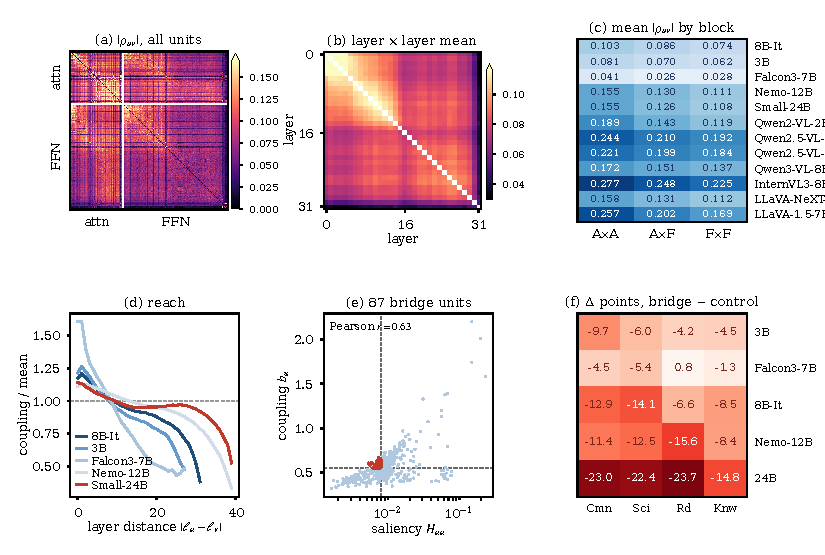
\includegraphics[width=\textwidth]{figures/fig_edge_anatomy.pdf}
\caption{\textbf{The anatomy of the edge matrix, and what ignoring it costs.} Curvature correlation
$|\rho_{uv}|=|\Hmat_{uv}|/\sqrt{\Hmat_{uu}\Hmat_{vv}}$ puts every entry on one scale.
\textbf{(a)} the estimated matrix, units ordered attention-then-FFN: the off-diagonal quadrants are
populated, not residual. \textbf{(b)} the same matrix averaged into layer$\times$layer cells: mass
persists far from the diagonal band and concentrates in the first half of the depth. \textbf{(c)} the
attention$\leftrightarrow$FFN block is $0.74$--$0.98$ times the mean of the two within-module blocks
on all five text-only models, and $\vlmAFLo$--$\vlmAFHi$ on the \vlmStructN\ vision--language
models (rows marked VL), which the estimator was never specialised for. \textbf{(d)} coupling by layer distance, normalised so $1.0$ is the average pair.
\textbf{(e)} saliency against coupling, one point per unit; red is the bridge corner. \textbf{(f)}
matched-pair test: points lost by forcing the bridge corner out against a control matched on
saliency, unit type and cost, with one greedy fill shared by both arms. Twenty cells, five models,
nineteen negative; the colour scale spans the full range, so the largest model's cells dominate it and
the exact value is printed in every cell.}
\label{fig:anatomy}
\end{figure}

\textbf{The interactions node-first scoring discards are the same size as the ones it keeps.} The curvature correlation $|\rho_{uv}|$ puts every entry of $\Hmat$ on one scale, so the blocks are
directly comparable. The attention$\leftrightarrow$FFN block is not a correction term. It runs at
$0.74$ to $0.98$ times the mean of the two within-module blocks across five models
(\cref{fig:anatomy}c), and on Mistral-Nemo-12B it reaches $0.130$ against $0.155$ within attention. This is
the quantitative content of treating pruning as a joint operation across module types. It is also what
makes a \emph{shared} attention/FFN budget meaningful at all: without a term coupling the two types,
their saliencies live on incommensurable scales and any joint ranking is arbitrary.

\textbf{And they are not local.} Coupling peaks at a layer distance of zero or one, at $1.1$ to $1.6$
times the average pair, and decays slowly from there. It still stands at $0.33$ to $0.53$ of the average
across the full depth of the network (\cref{fig:anatomy}d), and the layer$\times$layer view shows it massed in the
first half of the depth (\cref{fig:anatomy}b), where every cell in the top decile of off-diagonal mass
lies.
A curvature model that is block-diagonal per layer, or confined to one module group, is therefore not
an approximation of this matrix that keeps most of its mass. It discards the part that spans the
residual stream.

\textbf{The structure names a minority of units.} Write $d_u=\Hmat_{uu}$ for a unit's own saliency
and $b_u=\sum_{v\neq u}|\Hmat_{uv}|$ for its total coupling. The two do not move together at the
bottom of the saliency range: $87$ of $768$ units on Llama-3.1-8B-Instruct sit in the low-$d_u$,
high-$b_u$ corner of \cref{fig:anatomy}e, and that corner holds under $15\%$ of units on every one of
the ten models ($3.5$ to $14.5\%$). A diagonal selector sees only $d_u$ and removes them early.
\method sees the second sum in \cref{eq:marginal} grow as their partners are taken, and holds them
back. These are \emph{bridge} units.

\textbf{What the diagonal cannot see is where a unit sits.} Coupling falls with depth
on every one of the ten models: the rank correlation $\rho_s(\ell_u, b_u)$ between a unit's layer
index and its coupling runs from $-0.54$ to $-0.91$, median $-0.87$, and is negative on $10$ of $10$.
Saliency carries no such signal. Its $|\rho_s|$ has median $0.18$, and the \emph{sign} is positive on
five models and negative on five (\cref{tab:depth-grading}). Depth is therefore not a weak feature of
node saliency, it is absent from it, and it is present in the off-diagonal at close to four times the
rank strength (median ratio $3.9\times$). That is what makes the bridge corner an early-layer population: coupling and depth are
close to the same axis, and the corner is where low saliency meets high coupling. It is also why the
allocation below is not a heuristic we imposed. The solver holds the early layers back because the
second sum in \cref{eq:marginal} is largest there.

\textbf{Deleting exactly those units reproduces the damage.} Structure in $\Hmat$ is not yet evidence
about the model, so we force the issue, on every model we build $\Hmat$ for. We prune the bridge units
outright against a control matched unit-for-unit on saliency, unit type and parameter cost but drawn
from the low-coupling population. One greedy fill, computed once and shared by both arms, completes
them, so the two masks hold the same number of units, the same attention/FFN split and the same
removed cost to the last bit, and differ only in which low-saliency population was forced out. On
Llama-3.1-8B-Instruct commonsense falls $12.9$ points, science $14.1$, world knowledge $8.5$ and
reading $6.6$ --- and WikiText perplexity \emph{improves} by $4.5$.

That dissociation is the mechanism in its sharpest form, and it is not one model's accident. Across
five models, nineteen of the twenty capability cells fall, by up to $23.7$ points, and the largest
model gives the largest effect: on Mistral-Small-24B all four groups fall by $14.8$ to $23.7$
(\cref{fig:anatomy}f, per-model numbers in \cref{tab:bridge-models}). On three of the five,
perplexity moves the other way while every capability group in that row falls, so the arm a
next-token proxy prefers is the arm that has lost the most capability. The claim is not that
perplexity always points the wrong way --- on Mistral-Small-24B the bridge removal costs $425$
perplexity as well, and there the two agree --- but that nothing makes it point the right way, and on
the majority of models here it does not. What node-first scoring mis-reads is not how important a unit
is on its own but what it is holding together, and the proxy such scoring is built on cannot be relied
on to notice. This is also why \cref{sec:exp-main} reports the two families side by side rather than
leading with the one our objective is closest to: the same caution applies to our own numbers, and the
capability columns are the ones we ask to be believed.

\begin{figure}[t]
\centering
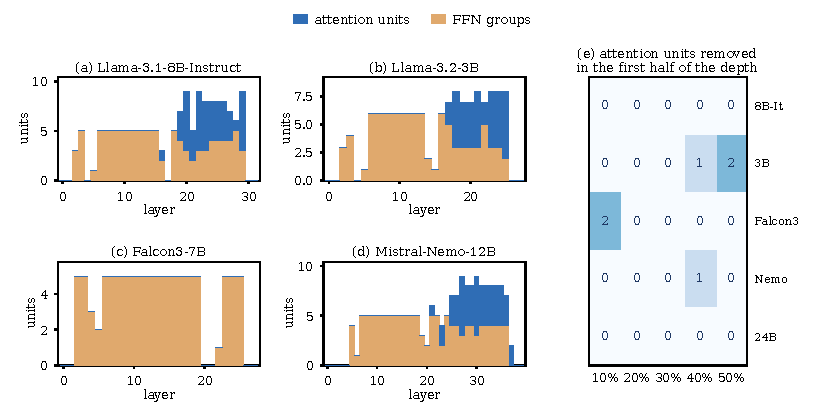
\includegraphics[width=\textwidth]{figures/fig_allocation.pdf}
\caption{\textbf{What one shared budget decides on its own}, read off the deployed solutions.
\textbf{(a)--(d)} per-layer, per-type removal at $\rho{=}20\%$: the first half of the depth is spent
entirely on FFN width and attention is touched only beyond it; on Falcon3-7B the objective declines to
remove attention anywhere. \textbf{(e)} the same quantity over five models and five ratios: eight of the
twenty-five solutions remove no attention anywhere, and of the seventeen that do, thirteen remove
\emph{exactly zero} from the first half and no exception exceeds two units. Mistral-Small-24B is not on
the machine that produced (a)--(d); its counts come from the same deployed masks. Nothing imposes this; the guard constrains only per-layer totals.}
\label{fig:allocation}
\end{figure}

\textbf{Given one budget, the objective writes its own allocation, and writes the same one every
time.} Methods in this literature fix the attention/FFN split by hand, or prune the two types in
separate stages. We fix nothing beyond the guard, and what comes out is not ``some of each everywhere''
(\cref{fig:allocation}). The first half of the depth is pruned \emph{entirely} out of FFN width. Not
one attention unit is removed before layer $17$ of $32$ on Llama-3.1-8B-Instruct, layer $18$ of $28$ on
Llama-3.2-3B, or layer $22$ of $40$ on Mistral-Nemo-12B, counting from one. Attention then takes close
to half of the removals over the second half ($50\%$, $49\%$, $45\%$) --- while on Falcon3-7B and
Mistral-Small-24B the objective declines to touch attention at all. This is not a property of one operating point. Of the
twenty-five solutions over five models and five ratios, eight remove no attention anywhere, and the
other seventeen remove it only late: thirteen of those seventeen take \emph{exactly zero} attention
units from the first half of the depth, and the remaining four take one or two
(\cref{fig:allocation}e). Early attention is what the residual stream is built on. A criterion that
never sees the coupling between module types has no way to discover that, and here it falls out of a single minimisation in five
models spanning three distinct attention geometries: $(24,8,128)$, $(12,4,256)$ and
$(32,8,128)$ query heads, KV heads and head dimension.

\textbf{What this asks of the field.} Structured pruning has spent its effort on better node scores,
and a term none of them contain sets the ceiling on that programme. The pair term is measurable in any
dense Transformer, it costs one ablation per unit and no gradients, and the units it protects can be
located in a model before anything is pruned. The question to ask is not which units matter, but which
units matter \emph{together}. The object of study that follows is the matrix, not the ranking.

